\documentclass[a4paper, 11pt]{article}
\usepackage{graphicx}
\usepackage[a4paper,bindingoffset=0in,%
            left=1in,right=1in,top=1in,bottom=1in,%
            footskip=.25in]{geometry}
\usepackage[square, numbers]{natbib}

\begin{document}

\title{A Software Package for Extendable Decision Trees in C++}

\begin{titlepage}
	\centering
	\vspace{1cm}
	{\scshape\LARGE Ludwig-Maximilians-Universität München \par}
	\vspace{1.5cm}
	
\includegraphics[width=0.35\textwidth]{figure/lmu_logo.png}\par\vspace{1cm}
	\vspace{0.5cm}
	{\scshape\Large Bachelor Thesis in Computer Science\par}
	\vspace{1.5cm}
	{\huge\bfseries treelib - A Software Package for Extendable Decision Trees in C++\par}
	\vspace{2cm}
	{\Large\itshape Christian Alexander Scholbeck\par}
	\vfill
	supervised by\par
	Prof. Dr. Bernd Bischl \par
	Prof. Dr. Marvin Wright \par
	Dr. Giuseppe Casalicchio

	\vfill

% Bottom of the page
	{\large Month Day, 2021 \par}
\end{titlepage}

\newpage
\thispagestyle{empty}

\vspace*{4cm}
\begin{abstract}
This thesis provides a software package for extendable decision trees written in C++. The package follows object-oriented and modular design principles. It works as a standalone application, or can be called by other programming languages. It supports both binary and multiway splitting, and can be extended with new optimizing algorithms, split criteria, models, and objectives. Supported application areas include classic predictive modeling with decision trees such as CART or C4.5, and advanced modeling such as model-based recursive partitioning. Furthermore, the modular design principle allows the extension of the package to support novel applications such as surrogate modeling for interpretable machine learning.

\end{abstract}
\vspace{2cm}
\tableofcontents
\clearpage
\setcounter{page}{1}
\section{Introduction}

Decision trees are one of the most fundamental techniques in machine learning. They are frequently preferred over more complex models due to their intelligibility in the form of decision rules, e.g., in medical applications \cite{podgorelec_trees_medicine}. Tree learning algorithms are numerous and differ regarding split criteria, model choices, stopping rules and pruning. \par
Ideas for decision tree learning originate in supervised learning and date back as far as linear discriminant analysis \cite{fisher_lda}. A large variety of decision tree algorithms has been published, such as Automatic Interaction Detection (AID) \cite{hawkins_AID}, Theta AID \cite{ messenger_mandell_thaid}, Chi-Squared AID \cite{kass_chaid}, Classification and Regression Trees (CART) \cite{cart_1, hastie_elemstatlearn}, C4.5 \cite{quinlan_c45}, and many more \cite{loh_trees_review}.
\par
So-called hybrid, model, or functional trees \cite{zeileis_mob} have added capabilities such as fitting node models \cite{quinlan_model_tree}, or using linear combinations of variables for splits \cite{brodley_multivariate_trees}. Hybrid trees are also capable of unsupervised learning, e.g., by training kernel density estimators inside the nodes \cite{ram_density_estimation_tree}.
Recent developments have embedded hybrid trees into frameworks for  statistical inference, e.g., conditional inference trees \cite{hothorn_ctree} and model-based recursive partitioning (MOB) \cite{zeileis_mob}.
\par
A critical drawback of decision trees is a high variance under perturbations of the training data \cite{hastie_elemstatlearn}. This has led to the development of tree ensembles such as random forests \cite{breiman_randomforests}, which reduce variance to the detriment of losing interpretability.

%Popular variants include classification and regression trees (CART) \cite{cart_1}, C4.5 \cite{quinlan_c45}, and model-based recursive partitioning \cite{zeileis_mob}.
\par
%Their most critical drawback is a high variance under perturbations of the training data \cite{hastie_elemstatlearn}. This has led to the development of tree ensembles such as random forests \cite{breiman_randomforests}, which reduce variance to the detriment of losing interpretability.

%such as CART minimize the sum of squared deviations from the mean target value for regression tasks, or Gini impurity for classification tasks. More complex variants such as MOB train predictive models inside the leaf nodes, e.g., (generalized) linear models. Most decision tree variants such as CART or MOB are restricted to binary splits, whereas others such as C4.5 enable multiway splitting, which increases computational complexity.
%\par
%The possibilities of applying decision trees in contexts other than such as interpretable machine learning are numerous. For instance, due to their intelligibility, decision trees are especially suited as a surrogate model for black box models, where the black box predictions are approximated by interpretable functions inside the leaf nodes.
\par
Applications for decision trees are diverse, e.g., predictive modeling \cite{hastie_elemstatlearn}, surrogate modeling \cite{schaaf_surrogate_tree}, or density estimation \cite{ram_density_estimation_tree}. This creates a requirement for an accessible, efficient, and extendable software implementation of decision trees. Accessible, to benefit a broad scientific community. Efficient, as the computational demand of optimizing splits grows considerably with the tree's complexity. Extendable, as different applications require different decision tree setups.
\par

\subsection{Contributions} The central contribution of this thesis is a from-the-ground-up implementation of extendable decision trees as an open-source software package. The package is written in \texttt{C++} to achieve a high degree of computational efficiency, while preserving object-oriented principles and portability to other programming languages. The package follows modular design principles to achieve a maximum degree of extensibility.
\par
The written thesis provides a compact literature review of decision trees and smart splitting. Furthermore, it describes the software design and extensibility to support other applications, and demonstrates the package on simulated and real data.

\subsection{Software Description}

The software can be run as a standalone application, and supports console outputs of tree information such as the tree structure, and node summaries. Furthermore, it can be called by other programming languages for the usage in more flexible application environments. The program specifications are determined at runtime. It supports an arbitrary number of splits.
The package is equipped with two types of objective functions; sum of squared errors (SSE) for regression tasks, and the Gini impurity for classification tasks. Node models include: majority vote (classification), mean target value (regression), and linear regression model (regression and classification).
The modular structure allows for the extension with 
new optimizing algorithms, split criteria, node models, and objectives. 

\section{Related Work}

An initial software implementation of MOB was published as part of the \texttt{party} package \cite{party_package} for the \texttt{R} programming languge for statistical computing \cite{r_citation}. A more flexible version, which supports more inference options and is extendable to new models, was introduced in the \texttt{partykit} package \cite{partykit_package}. 
\par
The \texttt{R} language is able to directly call \texttt{C} or \texttt{C++} code, which warrants significant speedups in computational execution time \cite{eddelbuettel_rcpp}. However, software implementations which are solely written in \texttt{R} code such as \texttt{partykit} pose a considerable bottleneck in computational speed.
The software package \texttt{ranger} \cite{ranger_package} provides a fast implementation of random forests in \texttt{C++} and can be directly called from the identically named \texttt{R} package. However, it is restricted to random forests and intextendable regression trees.

\section{Theory}

Decision tree learning algorithms recursively partition the data through greedy optimization of an objective function. Subsequent partitionings can be visualized as a series of decision rules, which together form a tree graph (see Fig. \ref{fig:tree_structure}). Each partitioning of the data is referred to as a node, whereas a final partitioning is referred to as a leaf node. The starting point of a decision tree, which encompasses the entire, unpartitioned data, corresponds to the root node. When decision trees are used for predictive modeling, they are commonly referred to as regression trees for continuous target variables, and classification trees for categorical ones.

\begin{figure}
    \centering
    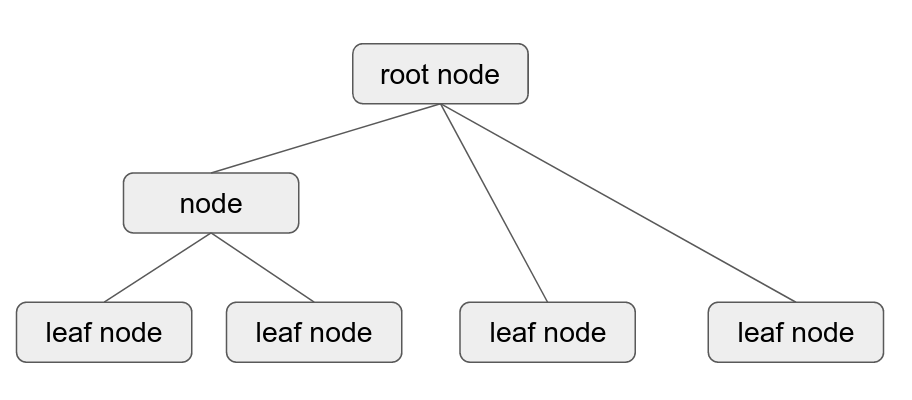
\includegraphics[width = 0.6 \linewidth]{thesis/figure/tree_structure.png}
    \caption{General decision tree structure comprising a root node, regular nodes, and leaf nodes.}
    \label{fig:tree_structure}
\end{figure}





%\par
%Training more complex models inside the nodes such as (generalized) linear models increases the predictive performance of the decision tree, but increases computational costs. Training a complex model for every potential split is infeasible in practice. 


% \subsection{General Setup}

% Each decision tree has five common components:
% \begin{enumerate}
%     \item \textbf{Node model choice:} A node model can be of any type.
    
%     e.g., none (if the objective does not require predictions), a constant, a (generalized) linear model, or a kernel density estimate. The model type can vary across nodes.
%     \item \textbf{Objective function:} 
%     The objective function determines the selection of a split. Its characteristics depend on the purpose of the decision tree, e.g., the L2 loss for predictive modeling, or the integrated squared error for kernel density estimation \cite{ram_density_estimation_tree}. The objective may vary across nodes, e.g., computational costs can be decreased by using a heuristic for initial splits with many observations. 
%     \item \textbf{Optimization:} For each node, we need to find one or multiple split points that improve the objective given certain hyperparameters such as the minimum node size.
%     \item \textbf{Stopping:} We may either split the tree down as far as possible, or use an early stopping criterion.
%     \item \textbf{Pruning:} To avoid overfitting, the tree can be pruned post-hoc.
% \end{enumerate}

\par
With a growing complexity, e.g., due to the cost of training node models for every split or multiway splitting, the computational cost of decision trees grows considerably. This puts a great importance on an efficient split search, which can be achieved in multiple ways.
First, computations can be parallelized, e.g., after splitting a node, the computations in all child nodes are independent of each other and can run in parallel.
Second, we can evaluate a subset of values, e.g., if the split variable is continuous, close values can be omitted from the search.
Third, for each node there is a large number of split points to be evaluated. Instead of recomputing the objective for each split, computations may be sped up by an update mechanism.
Fourth, an intelligently constructed split point generator can suggest split points with a higher probability of improving the objective than others.
\par
In the following, we explore the third and fourth option, i.e., update mechanisms for objective functions and split point generation.

\subsection{Updating Objective Functions}

\subsubsection{Total Sum of Squares}
CART is a commonly used decision tree variant \cite{hastie_elemstatlearn}, which does not train models inside the leaf nodes. For regression trees, CART minimizes the weighted sum of squared deviations between the child node target values and the corresponding mean value, i.e., the total sum of squares (TSS). The TSS is equivalent to the sum of squared errors (SSE) if the trained model corresponds to the mean target value.
For classification trees, CART minimizes Gini impurity, which summarizes the distribution of relative target class frequencies. 
%CART is restricted to binary splits. The tree is fully grown until a pre-specified minimum node size criterion would be violated when splitting further. The tree height is pruned post-hoc according to a complexity parameter to avoid overfitting, which is estimated via cross-validation. Missing values are handled via surrogate splits.


%\par
%C4.5 is similar to CART, but is restricted to classification trees. It uses an information-theoretic measure of node impurity called gain ratio, which corresponds to the quotient between information gain and entropy. C4.5 conducts multiway splits for categorical variables, i.e., all observations of the same category are binned together. Additional differences between CART and C4.5 can be found for missing values, which requires surrogate splitting.
\par
Consider a binary split which partitions a node into two subsets with $n_1$ and $n_2$ observations, and child node TSS $L_1$ and $L_2$. The left node TSS with $n_1$ observations and target vector $y_1$ can be decomposed as:
$$
L_1^{(0)}(y_1) = \sum_{i = 1}^{n_1} \left(y_1^{(i)} - \overline{y_1}\right) = \sum_{i = 1}^{n_1} \left(y_1^{(i)}\right)^2 - \sum_{i = 1}^{n_1} y_1^{(i)} 
$$
For the next split value, there are two different partitionings with either $n_1 + 1$ and $n_2 - 1$, or $n_1 - 1$ and $n_2 + 1$ observations. For the first option, the loss can be updated as:
$$
L_1^{(1)}(y_1) = L_1^{(0)} + y_{1}^{(n_1 + 1)} - y_{1}^{(n_1 + 1)}
$$
For the second option, it can be updated as:
$$
L_1^{(1)}(y_1) = L_1^{(0)} - y_{1}^{(n_1)} + y_{1}^{(n_1)}
$$


\subsubsection{Linear Model Trees}

The algorithm M5 \cite{quinlan_model_tree} was the first extension of ordinary decision trees to incorporate leaf node models.
M5 starts with growing a decision tree by selecting splits that minimize the standard deviation of target values. It then adds linear regression models to the leaf nodes, and prunes the tree. 
\par
Training linear leaf node models, whereas the splits have been determined via reduction of target variance creates a discrepancy in model fit. In \cite{potts_incremental_model_tree}, the authors propose to incrementally estimate the leaf node models through each split.

\subsection{Split Point Generation}





\section{Software Design}

\section{Extensibility}

\section{Demonstrations and Benchmarks}

\section{Conclusion}
\bibliographystyle{plainnat}
\bibliography{bibfile}


\end{document}